\documentclass[english, 12pt]{article}

%import required packages
\usepackage[top=1in, bottom=1in, left=1in, right=1in]{geometry}
\usepackage{cite}
\usepackage{babel,blindtext}
\usepackage{graphicx}
\usepackage{caption}
\usepackage{subcaption}
\usepackage[utf8]{inputenc}
\usepackage{multirow}
\usepackage{hhline}
\usepackage{float}

%start the document
\begin{document}

%function to leave tab, named \tab
\newcommand\tab[1][1cm]{\hspace*{#1}}
\newcommand\spacet[1][1cm]

%title of the document
\title{\textbf{Landmine - Rock or a Mine Detection}}
\author{
	\begin{large}
		Landmine group
	\end{large} \\
		Biometrics and Machine Learning Lab\\
		University of Florida
	}
\date{\today}
\maketitle

%abstract of the document
\begin{Large}
	\begin{center}
		\textbf{Abstract} 
	\end{center}
	\end{Large}
\begin{large}
\textit{\tab This report explicates usage of TUF software and lists comparative analysis of Feature extraction algorithms on various datasets. Data dealt with consists of signals through the earth's crust deflected by a mine or a rock. With steps of Prescreening, Feature Extraction and Machine Learning Classification we can provide a statistical probability of detecting a mine or a rock. This report examines observes features to vary prominently in shape over textures. Hence, feature-set, extracting spatial orientations outperform textural features.}
\end{large} 
\\

%keywords section
\textit{\textbf{Keywords:}  LBP- Local Binary Pattern, GRAB- Generalized Region Assigned to Binary, HOG-Histogram of Gradients, LESH- Local Energy Based Histogram, LPQ- Local Phase Quantization, WLD- Weber Local Descriptor, SVM- Support Vector Machines, GRNN- Generalized Regression Neural Network, RBF- Radial Basis Function, ROC- Receiver Operating Characteristic.} 

%introduction section
\section{Introduction}
\tab TUF software comes with inbuilt prescreeners,feature extractors, machine learning classifiers and embedded datasets. This report concentrates on feature extraction algorithms as applied to landmine dataset. Careful observation of data reveals that the data consists of signals with varying patterns distinguishing a rock and a mine. The inherent differences in the patterns can be captured by the feature extraction algorithms. Further, using machine learning classifiers, we can categorize input data pattern into a rock or a mine. In this report, we explore various extraction algorithms like LBP, GRAB, HOG, LESH, LPQ and WLD. Some of these extract features related to spatial orientations, while others to textures. Also, machine learning classifiers namely; SVM linear, SVM- RBF and GRNN, are used in the data classification. Comparative analysis is performed amongst the feature extraction algorithms and machine learning classifiers.

%methodology section

\section{Methodology}

%secton for feature extraction algorithms
\subsection{Feature Extraction}
\tab Feature extraction derives important information from the input data. Sometimes, only by discarding redundant 
feature values, is it possible to reduce the input dimension. Few extraction techniques focus on the texture, while others on spatial orientations. Amongst the feature extractors mentioned, LBP and GRAB extract textural pattern of the data, whereas, HOG, LPQ, LESH, and WLD extract spatial orientations.

%\begin{figure}[H]
%    \centering
%    \begin{subfigure}[b]{0.8\textwidth}
%        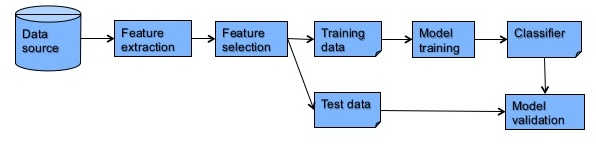
\includegraphics[width=\textwidth]{intro.jpg}
%    \end{subfigure}
%    \centering
%    \caption{Overview of Methodology}\label{fig:intro}
%\end{figure}

%first feature extraction algorithm: LPB
\subsubsection{LBP- Local Binary Pattern}
\tab The local binary pattern as described in \cite{Ahonen:2006:FDL:1175897.1176245} is useful to find textures such as edges, corners and other non-uniform variations .LBP is used in various applications like face detection, iris gender recognition. A characteristic feature of LBP is its dependence on the neighboring pixels. In evaluating LBP, 8 surrounding pixels of one selected pixel are considered. Traditional LBP is signed Compound–LBP. That is, neighboring pixels are compared in magnitude with pixel at the center. Figure \ref{fig:lbp} shows calculation of LPB value for the selected pixel.
\begin{figure}[h]
    \centering
    \begin{subfigure}[b]{0.55\textwidth}
        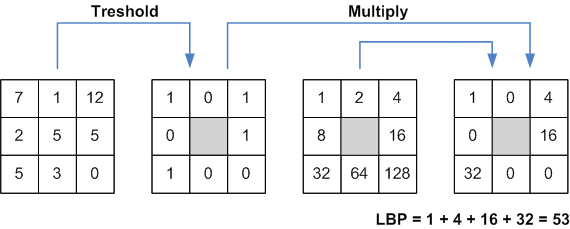
\includegraphics[width=\textwidth]{lbp.png}
    \end{subfigure}
    \centering
    \caption{Local Binary Pattern}\label{fig:lbp}
\end{figure}

\tab Let the value of center pixel be $g_c$ and the value of corresponding 8 neighboring pixels be $g_p$. Let $s(x)$ be 1 if $x >= 0$ else 0. Then,
\\
$$LBP = \sum_{n=0}^{7} s(g_c - g_p)2^n $$
\tab Windows extract more information as they are locally fixed around particular region. Similar consequence of overlapping windows suggests: information missed by non–overlapping windows is captured by overlapping windows. Thus while evaluating LBP features, we use 10x10 windows with 50\% overlap. Feature-set of LBP consists of concatenated histograms calculated for each of the overlapped window.

\subsubsection{GRAB- Generalized Region Assigned to Binary}
\tab While LBP is invariant to variables like illumination, translation, rotation, it may not be able to handle scale changes. GRAB deals with it by combining micro-structure and global structure, as well as the structure at multiple scales by extracting features at varying scales of the images. See Reference \cite{Sapkota2013}.
\\
\tab GRAB operator is applied on a Geo-normalized image. First, an averaging operator is applied to the image with the window size of $N/N$. For each $N/N$ region in the image, the center pixel of the region is assigned an average value of that region resulting in a smoothed image. Second, the neighboring operator such as LBP is applied to the smoothed image. In our experiments, we apply the averaging operator thrice with 3*3, 5*5, and 7*7 window size, and then apply Uniform-LBP on these images to get the feature set. 

\subsubsection{HOG-Histogram of Gradients}
\tab HOG is capable of characterizing local object and shape by calculating the local intensity gradients as shown in \cite{Dalal05histogramsof}. Here, each image is divided into connected regions called cells. Histogram of gradient directions of each cell is concatenated to produce the feature vector. Contrast normalization is carried out by grouping cells into blocks. In each block, histograms of cells are concatenated and normalized using L-2 norm, clipped L-2 norm,or L-1 norm. In our experiments we use L-1 norm. 
\\
\tab In the first step, use 1-D discrete derivative mask in the horizontal ($[-1, 0, 1]^T$) and the vertical ($[-1, 0, 1]$) direction. Calculate orientation based histogram for each cell. Orientations are observed to be signed $(0^{\circ}-180^{\circ})$ or unsigned  $(0^{\circ}-360^{\circ})$. Results indicate 9 bin histogram to be the best. For local normalization, cells are grouped into larger entities called blocks.
Histograms of these cells are concatenated to form block histograms. Block histograms are normalized using L-1 norm for illumination and contrast invariance.

\subsubsection{LESH- Local Energy Based Histogram}
\tab LESH as discussed in \cite{Wajid:2015:LES:2793715.2793763} is used to obtain an underlying shape description of the image. LESH accumulates local signal energy. Local histogram for image patches along several filter orientations are constructed. Histograms of patches are concatenated into a 128 dimensional spatial histogram. LESH is used in several applications like shape based image retrieval, object detection, and pose estimation.
\\
\tab In LESH, 	the input image is divided into 16 sub regions and each region is convolved with a bank of Log Gabor kernels along 5 scales and 8 orientations. The normalized energy value for each orientation is computed along all the scales. At 	each pixel position, the normalized energy values along each orientation is compared and a Label Map L is computed using the orientations of the maximum energy value. For all the 16 sub-regions, an 8 bin histogram is computed and concatenated to give a 128 	  bin histogram.

\subsubsection{WLD- Weber Local Descriptor}
\tab Feature descriptors are derived from Weber’s Law:
\textit{'if ratio of change to stimulus to original stimulus is large enough, the change can be recognized}'. WLD as explained in \cite{6166675} is computationally efficient and invariant to the illuminations. Differential excitation and orientation of textures are used to extract features. WLD computes salient micro patterns by differential excitation. Statistics of these patterns is built using gradient orientations at each pixel.

\begin{figure}[H]
    \centering
    \begin{subfigure}[b]{0.55\textwidth}
        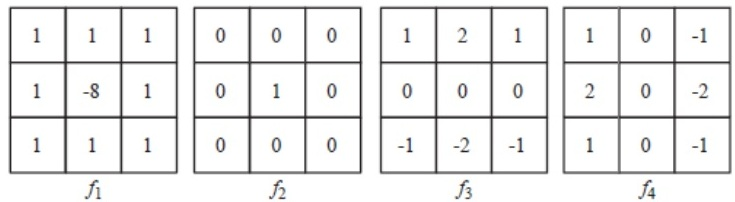
\includegraphics[width=\textwidth]{wld.jpg}
    \end{subfigure}
    \centering
    \caption{filters for Weber Local Descriptor}\label{fig:wld}
\end{figure}

\tab Compute the differential excitation by convolution of the image with filters f1, f2 to obtain v1, v2 respectively. Map the ratio of v1 to v2 to $[-\pi/2,\pi/2]$. Similarly, compute the differential orientation by convolution of the image with filters f3, f4 to obtain v3, v4 respectively. Map the ratio of v3 to v4 to $[-\pi/2,\pi/2]$. Quantize into 8 different orientations. Histogram of these values is calculated, which is the feature-vector for WLD. Refer Figure \ref{fig:wld} for f1, f2, f3 and f4 filter values.


\subsubsection{LPQ- Local Phase Quantization}
\tab LPQ Texture classifier is robust and invariant to image blur (refer \cite{Rahtu:2012:LPQ:2364628.2364653}). Phase information is computed locally in every image window, wherein, Phases of 4 low frequency components are computed, decorrelated, and quantized in 8 dimensional space. Histogram of resulting encoded values is computed and concatenated to form the feature vector.
\\
\tab LPQ computes the Short Term Fourier Transform (STFT) over a rectangular neighborhood at each pixel position. Complex coefficients corresponding to the 2-D frequencies are considered. At each position of the image window, a covariance matrix is computed. Covariance coefficients are decorrelated to maximally preserve information. Scalar quantization allows for information preservation in samples if they are statistically independent. Assuming a Gaussian distribution, statistical independence is achieved by applying a Whitening 	Transform at each image window position. For all the pixels in each window, quantization is carried out using a simple scalar quantizer. Quantized coefficients are represented as integers between 0-255 by binary coding. A 256 bin histogram of the binary encoded values of the entire image serves as the final feature vector.

\subsection{Machine Learning Classification}
\tab In the classification problem, we categorize a new observation into classes based on the training of past observations whose class is known. Different classifiers use their own characteristic algorithm to separate data. From the known Machine Learning classifiers, we use SVM and GRNN to classify our data into a rock or a mine.
\\ 
\tab In this report, we use SVM-linear, SVM-RBF and GRNN to train and test landmine features. The downside of using SVM-RBF and GRNN is the lack of data content. Thus, SVM-Linear is seen to produce higher classification accuracy over SVM-RBF or GRNN. While training and testing, we divide our data into ten cross-folds. Here, ${9/10}^{th}$ part of the data is trained and ${1/10}^{th}$ is used for testing. Likewise, data is trained and tested for a total of ten times, with each ${1/10}^{th}$ part of the data tested. Therefore, resulting accuracy for each ${1/10}^{th}$ part is found. In our results, average accuracy is the average of each of the cross-fold accuracy values.


%dataset section
\section{Datasets}
\tab TUF software consist of four datasets, of which three are fully functional for now. Additional datasets if added may contribute to much more reliable results. The three datasets used in our experiments are namely: MPGSept2005, Small Millbrook, and Tiny Millbrook. MPGSept2005 constitutes a total of 1791 input images of which 496 represents mine data. Small Millbrook and Tiny Millbrook are smaller datasets of  540 and 43 images respectively. Our experiments expose Tiny Millbrook to be too small to make any valid observations. The other two datasets are used to compare feature extraction and Machine learning algorithms. 

%result section
\section{Overview of Results}
\tab Firstly, we list out the results associated with various combinations of feature extraction techniques and machine learning classifiers. Secondly, feature level fusion is seen to improve the overall classification results. Thirdly, under discussion section, we present some insights which might further help in our future work. 

%first part of result section
\subsection{ROC- Receiver Operating Characteristic Curves}
\tab In this section various feature extraction techniques are evaluated. Due to the limitations on the size of the dataset, SVM- Radial Basis Function fails to produce substantial classification results. Hence, along with different feature extractors, SVM-Linear and GRNN are used in the experiments. Also, considering the size of datasets, we will focus on MPGSept2005 and Small Millbrook datasets and discard Tiny Millbrook dataset. A ten fold cross-validation technique is used, which facilitates in evaluating the data consistency.
\\
\tab Table~\ref{table:table1} lists results with different combinations of Classifier and Extractors.  In case of dataset MPGSept2005, for every feature extraction algorithm SVM-Linear outperforms GRNN classifier. LBP and GRAB extract the textural content of the data. However, shape based features helps to distinguish the data into a rock or a mine. Thereby, better classification accuracy can be observed using HOG or LPQ. Even though WLD and LESH are orientation dependent, small feature set result in poor classification accuracy, proving a tradeoff between the size of the feature-set and the classification accuracy. Overall for MPGSept2005, highest average of $93.29\%$ is achieved by using HOG feature extractor and SVM-Linear classifier. Also, lesser standard deviation suggests  extracted features to consistently differentiate the input data into their respective classes. Compared to all the feature extraction algorithms, HOG has the least standard deviation. Therefore, features extracted by HOG almost directly distinguish the input data into a rock or a mine. Few inferences made for MPGSept2005 don't hold true for Small Millbrook as it is a smaller dataset. However, similar to MPGsept2005, HOG and linear-SVM achieves highest average , alongside producing the least standard deviation. As a performance measure, ROC curves are plotted for the feature extractors of WLD, LESH, GRAB, LBP, LPQ and HOG (Refer Figure~\ref{fig:roc}). Highest GAR and lowest FAR define an ideal classification system. Tracing HOG curve will lead us to the highest GAR- Genuine Acceptance ratio and the least FAR- False Acceptance ratio. Thereby, HOG is a near ideal system, followed by LPQ.
\\
\\

\begin{table}[H]
\centering
		\caption{ Comparative analysis of feature extractors and Machine Learning Classifiers}
		\label{table:table1}
\centering
	\begin{tabular}{ |p{2.1cm}|p{1.6cm}|p{1.7cm} p{1.6cm}|p{1.7cm}|p{1.7cm}|p{1.7cm}|}
    	\hline
			\multicolumn{1}{|c|}{} & \multicolumn{1}{|c|}{}&
			 \multicolumn{3}{|c|}{\textbf{MPGSept2005}} & \multicolumn{2}{|c|}					{\textbf{Small Millbrook}}\\
		\hhline{~~-----}
			\multicolumn{1}{|c|}{\textbf{Feature}} & \multicolumn{1}{|c|}						{\textbf{\#}} &
			 \multicolumn{2}{|c|}{\textbf{SVM-Linear}} & \multicolumn{1}{|c|}					{\textbf{GRNN}} & \multicolumn{1}{|c|}{\textbf{SVM-Linear}} & 						\multicolumn{1}{|c|}{\textbf{GRNN}}
			 \\
		\hhline{~~-----}
			\textbf{Extractors} & \textbf{features} & 
			\textbf{mean \spacet accuracy} &
			\textbf{$\pm$std dev} &
			\textbf{mean \spacet accuracy} &
			\textbf{mean \spacet accuracy} &
			\textbf{mean \spacet accuracy}\\
		\hline
		\hline
			WLD & 1x80  & 60.22  & $\pm$18.61 & 64.19 & 76.85 & 76.48\\
		\hline
			LESH & 1x128 & 72.29 & $\pm$18.60 & 72.29 & 82.96 & 82.96\\
		\hline
			GRAB & 1x101598 & 76.59 & $\pm$14.48 & 67.98 & 83.88 & 76.48\\
		\hline
			LBP & 1x146944 & 78.04 & $\pm$14.56 & 75.53 & 85.18 & 80.92\\
		\hline
			LPQ & 1x24600 & 82.68 & $\pm$11.96 & 72.29 & 83.33 & 82.96\\
		\hline
			HOG & 1x7200 & 93.29 & $\pm$5.24 & 87.09 & 91.48 & 87.03\\
		\hline
	\end{tabular}
\end{table}

\begin{figure}[H]
    \centering
    \begin{subfigure}[b]{1\textwidth}
        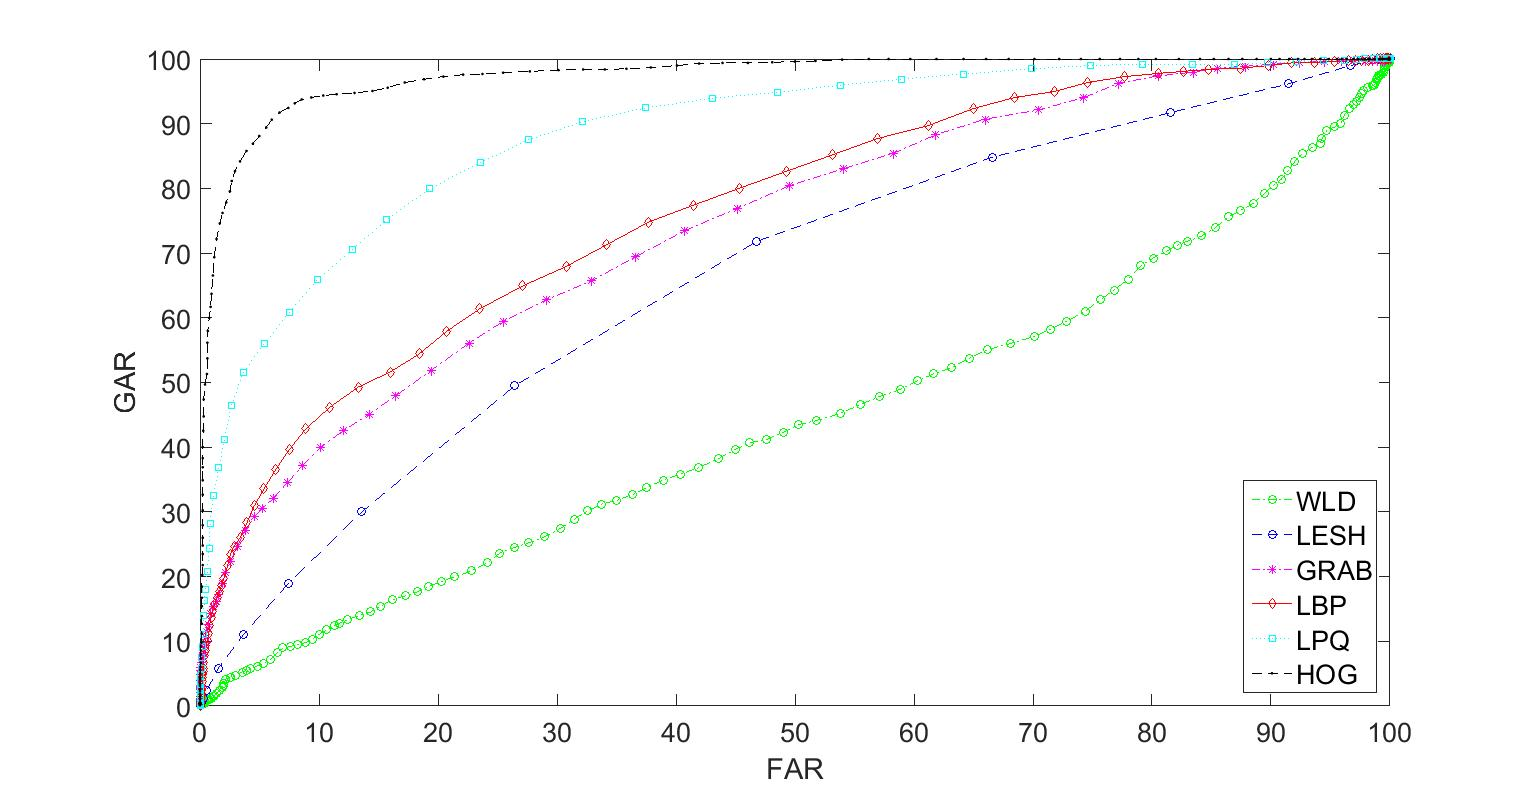
\includegraphics[width=\textwidth]{roc1_better.jpg}
        \label{fig:cproc}
    \end{subfigure}
    \centering
    \caption{Receiver Operating Characteristic curves for WLD, LESH, GRAB, LBP, LPQ, and HOG. }\label{fig:roc}
\end{figure}

%second part of resut section
\subsection{Feature level Fusion}
\tab There are various levels of fusion. Of these, feature level fusion is the raw concatenation of features extracted using different algorithms. For MPGSept2005 dataset, HOG turned out to be the best feature extractor. We fuse HOG with other feature extractors like LBP, LPQ and LESH. All these results are noted using Linear-SVM as the classifier.   
\\
\tab Classification values of fused features can be referred from Table~\ref{table:table2}. The second best feature extractor was found to be LPQ. Therefore, combination of HOG and LPQ features produces the best average accuracy of $93.96\%$. Fusion of HOG and LBP doesn't seem to improve the classification results. Whereas, the fusion of HOG and LESH has an improved performance. The important reason behind this trend might be the size of the feature set. In feature level fusion, the bigger the size of one feature set, lesser is the contribution of other feature sets. This point can be proven true only by using other larger datasets. Figure~\ref{fig:crocf} shows ROC curves for HOG+LPQ, HOG+LPQ+LESH , HOG+LESH, and HOG+LBP. HOG+LBP is found to have the least system performance.

\begin{table}[H]
\centering
		\caption{Comparative analysis of fused features}
		\label{table:table2}
\centering
	\begin{tabular}{ |p{3cm}|p{3cm}|p{2.5cm} p{2.5cm}|}
    	\hline
			\multicolumn{1}{|c|}{\textbf{Feature}} & \multicolumn{1}{|c|}						{\textbf{\#}} &
			 \multicolumn{2}{|c|}{\textbf{MPGSept2005}} \\
		\hhline{~~--}
			\centering\textbf{Extractors} & \centering\textbf{features} & 
			\textbf{average \spacet accuracy} &
			\textbf{$\pm$standard \spacet deviation} \\
		\hline
		\hline
			HOG + LBP & 1x154144 & 78.32 & $\pm$14.36 \\
		\hline
			HOG + LESH & 1x7328 & 93.24 & $\pm$5.32 \\
		\hline
			HOG + LPQ + LESH & 1x31928 & 93.91 & $\pm$5.65 \\
		\hline
			HOG + LPQ & 1x31800 & 93.96 & $\pm$5.54 \\
		\hline
	\end{tabular}
\end{table}

\begin{figure}[H]
    \centering
    \begin{subfigure}[b]{1\textwidth}
		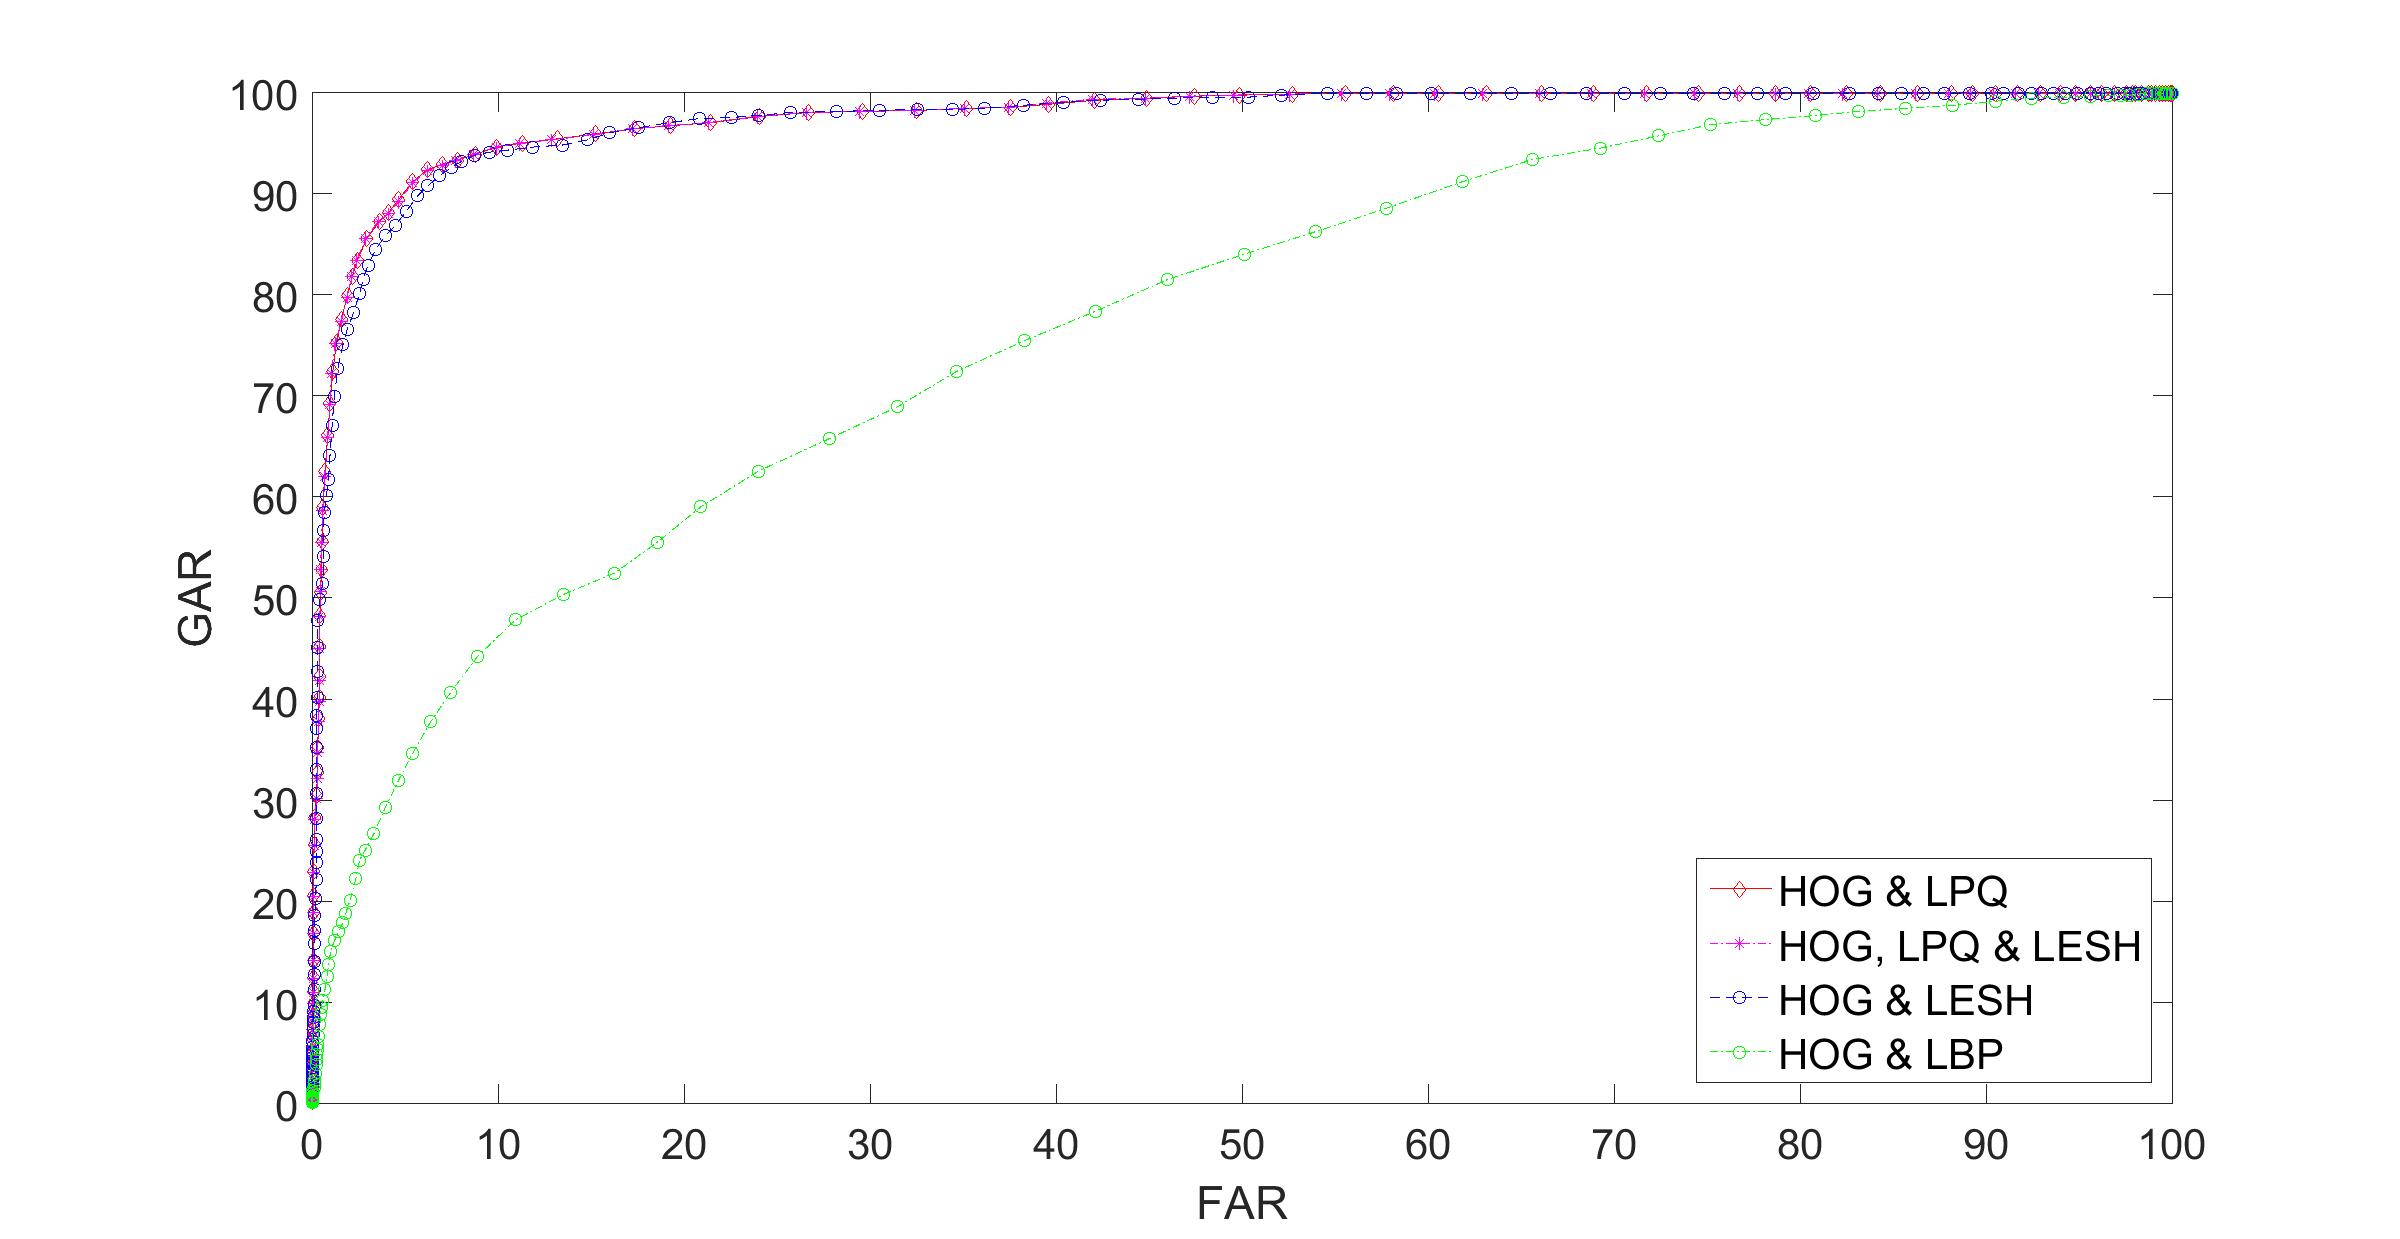
\includegraphics[width=\textwidth]{rocfusion.jpg}
	\end{subfigure}
	\centering
    \caption{ROC plots of fused features}\label{fig:crocf}
\end{figure}


\begin{figure}[H]
    \centering
    \begin{subfigure}[b]{0.44\textwidth}
        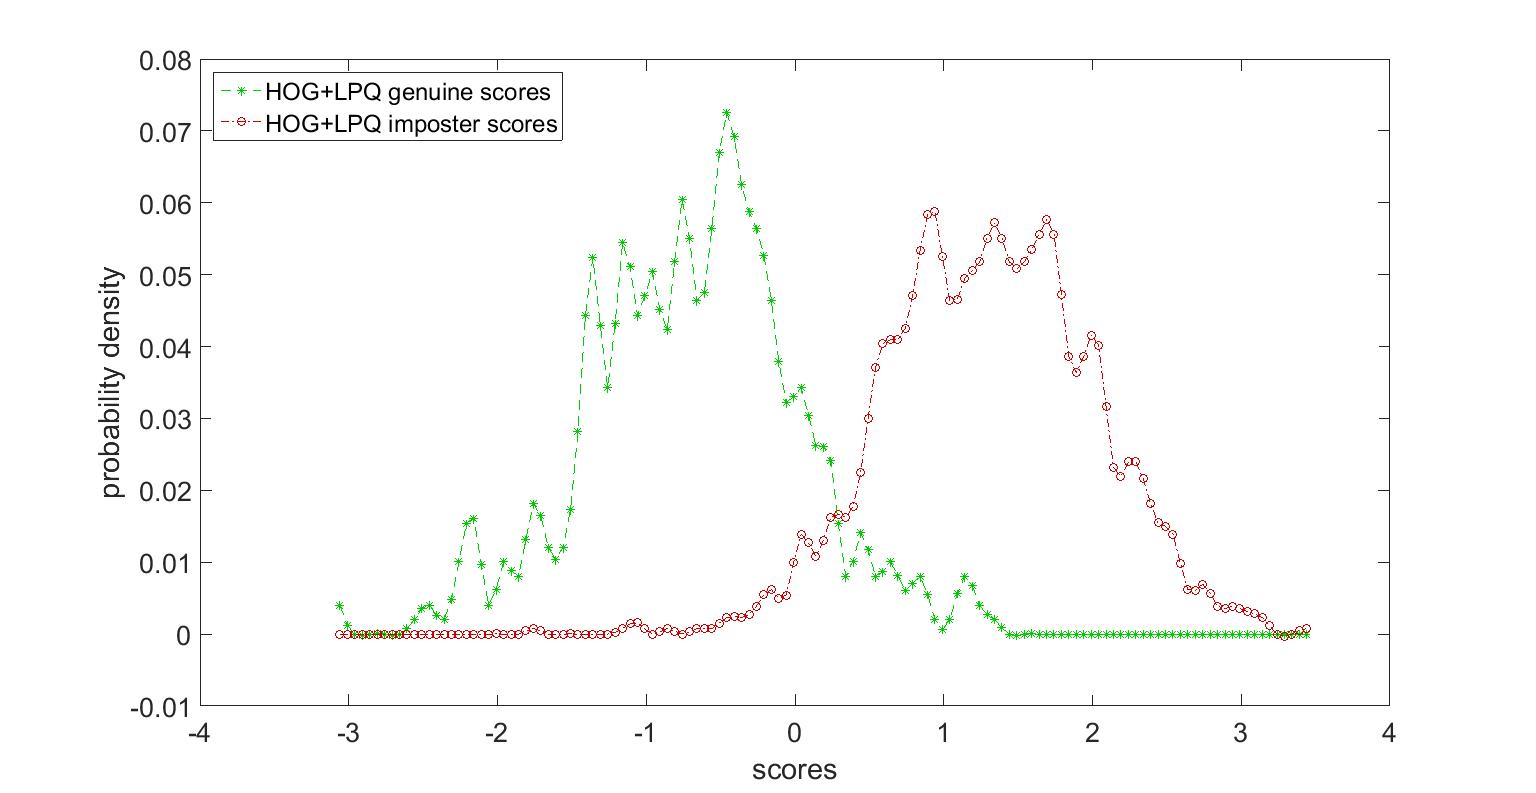
\includegraphics[width=\textwidth]{HOG+LPQ.jpg}
        \caption{HOG+LPQ = $93.96\%$}
        \label{fig:HOGLPQ}
    \end{subfigure}
    \begin{subfigure}[b]{0.44\textwidth}
        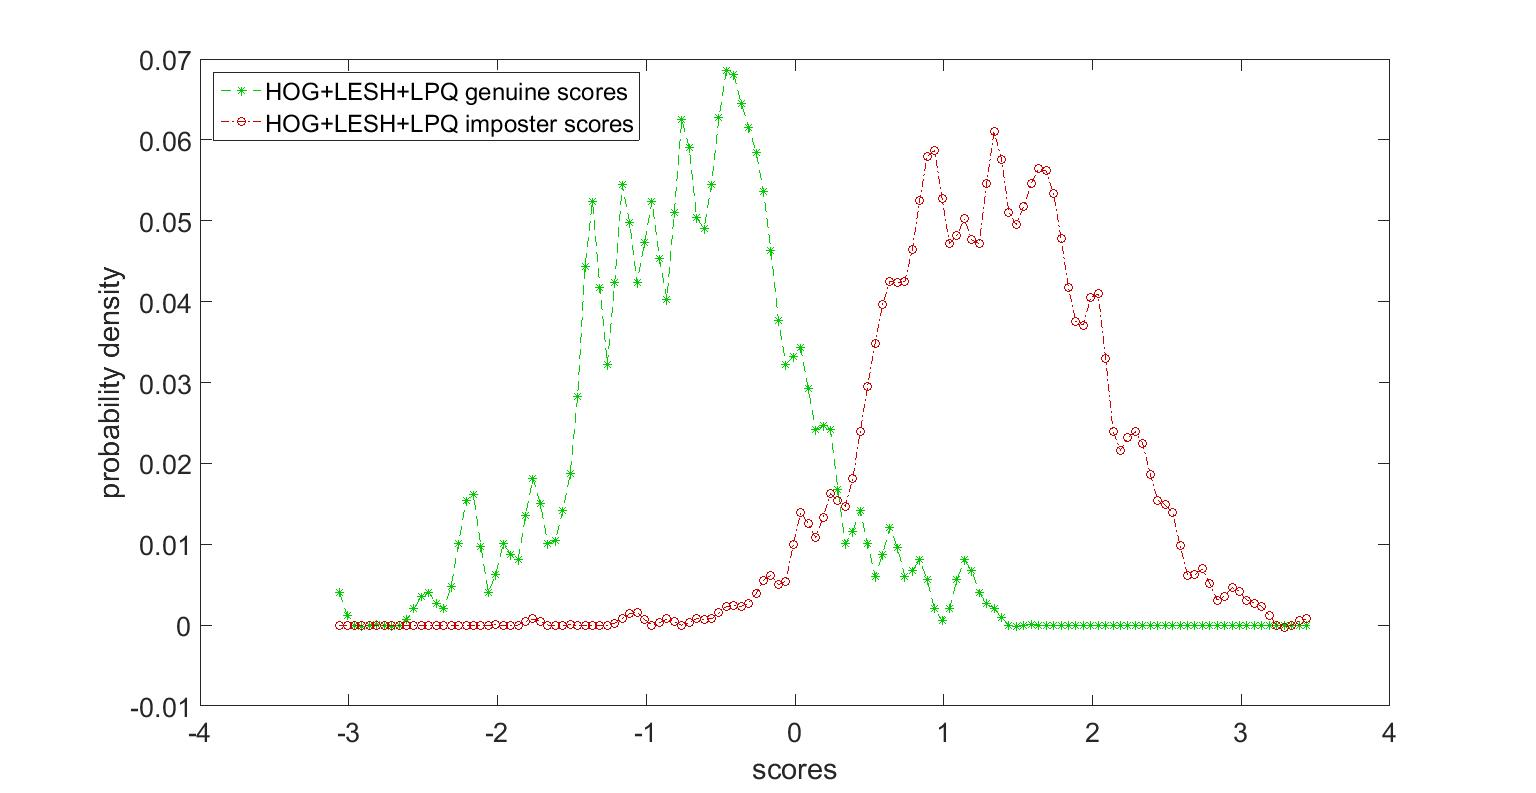
\includegraphics[width=\textwidth]{HOG+LPQ+LESH.jpg}
        \caption{HOG+LPQ+LESH = $93.91\%$}
        \label{fig:HOGLPQLESH}
    \end{subfigure}
    \begin{subfigure}[b]{0.44\textwidth}
        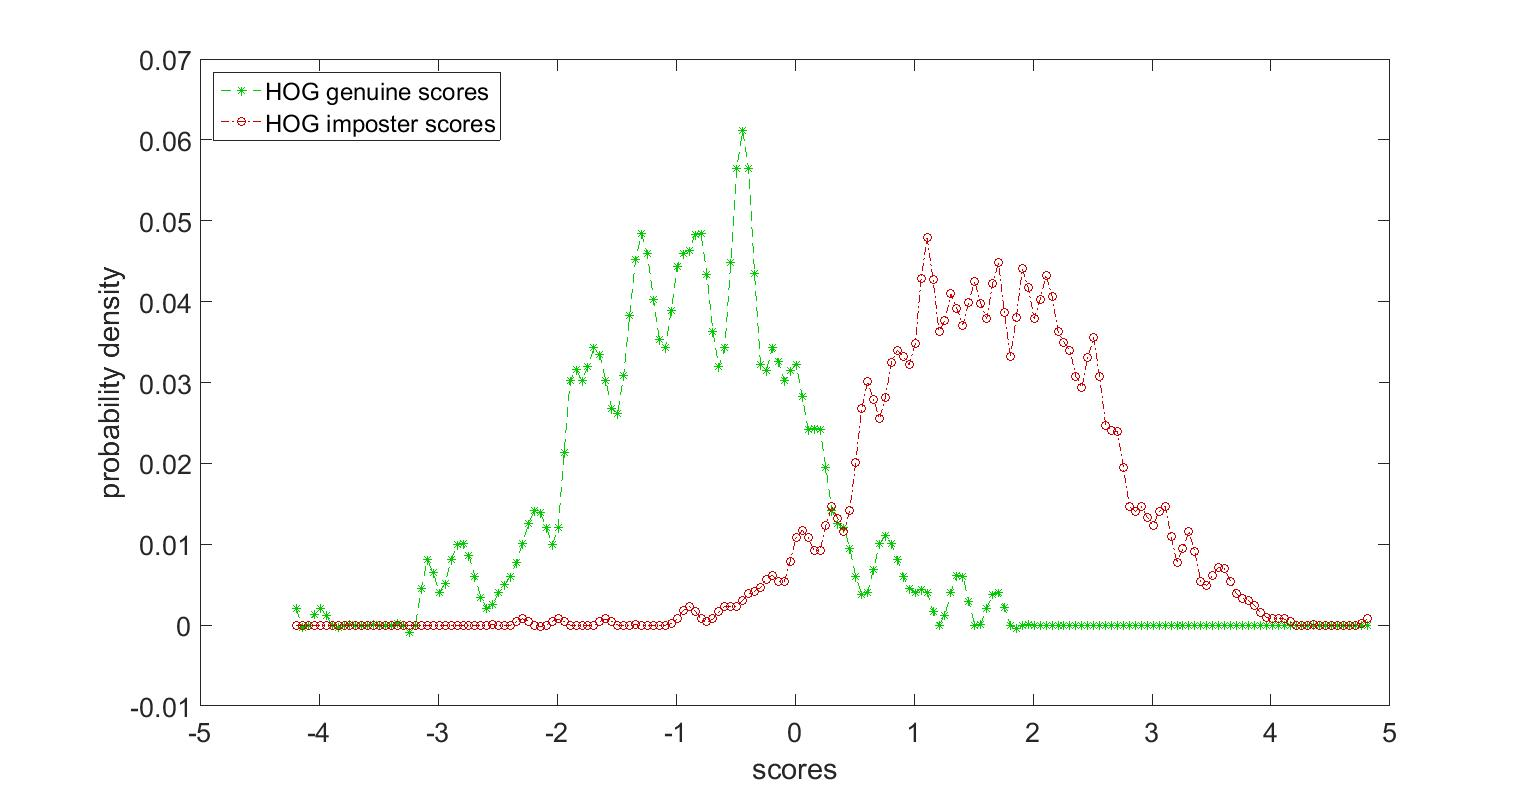
\includegraphics[width=\textwidth]{HOG.jpg}
        \caption{HOG = $93.29\%$}
        \label{fig:HOG}
    \end{subfigure}
    \begin{subfigure}[b]{0.44\textwidth}
        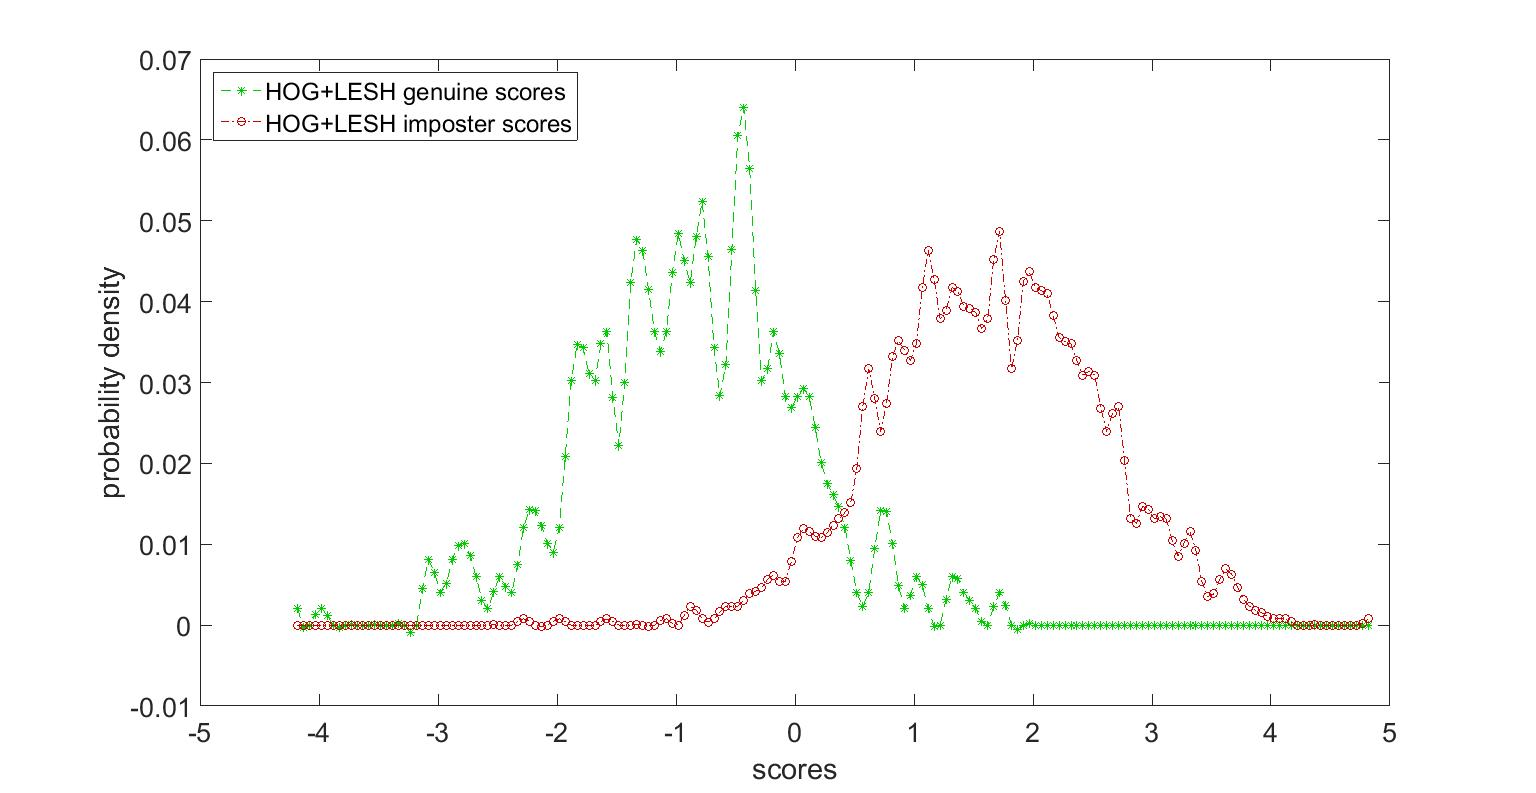
\includegraphics[width=\textwidth]{HOG+LESH.jpg}
        \caption{HOG+LESH = $93.24\%$}
        \label{fig:HOGLESH}
    \end{subfigure}
        \begin{subfigure}[b]{0.44\textwidth}
        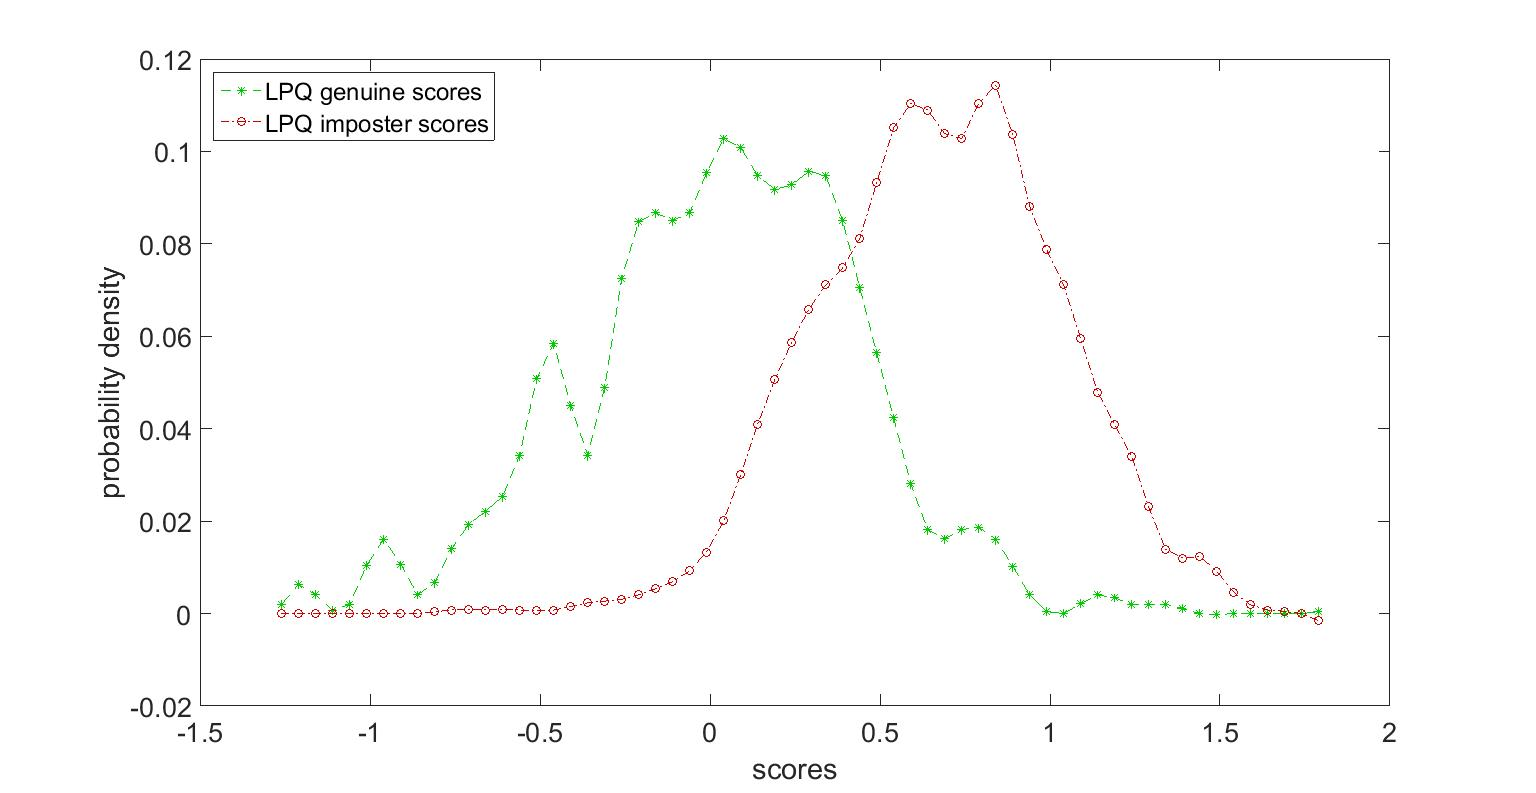
\includegraphics[width=\textwidth]{LPQ.jpg}
        \caption{LPQ = $82.68\%$}
        \label{fig:LPQ}
    \end{subfigure}
    \begin{subfigure}[b]{0.44\textwidth}
        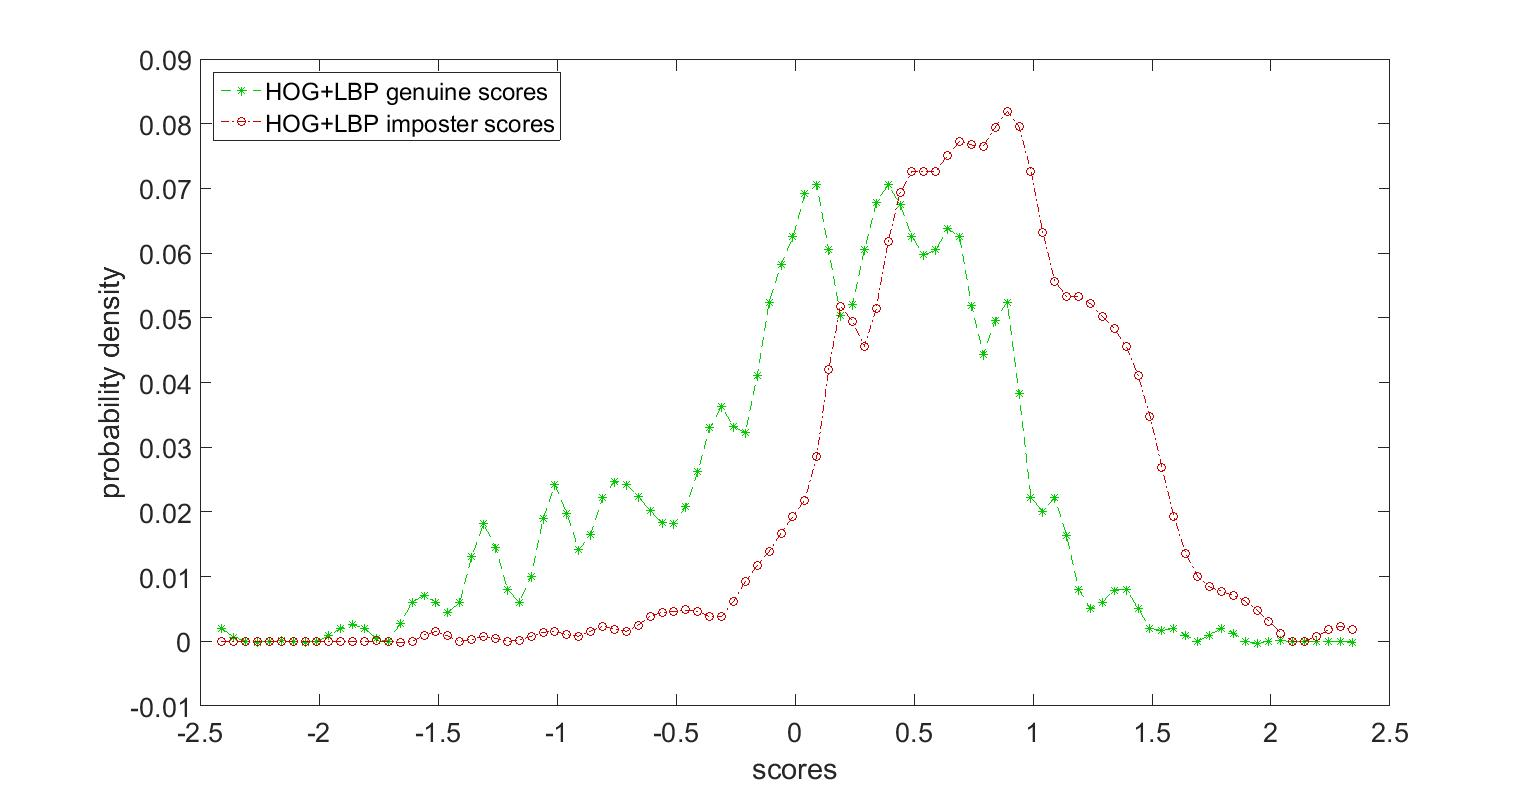
\includegraphics[width=\textwidth]{HOG+LBP.jpg}
        \caption{HOG+LBP = $78.32\%$}
        \label{fig:HOGLBP}
    \end{subfigure}
    \begin{subfigure}[b]{0.44\textwidth}
        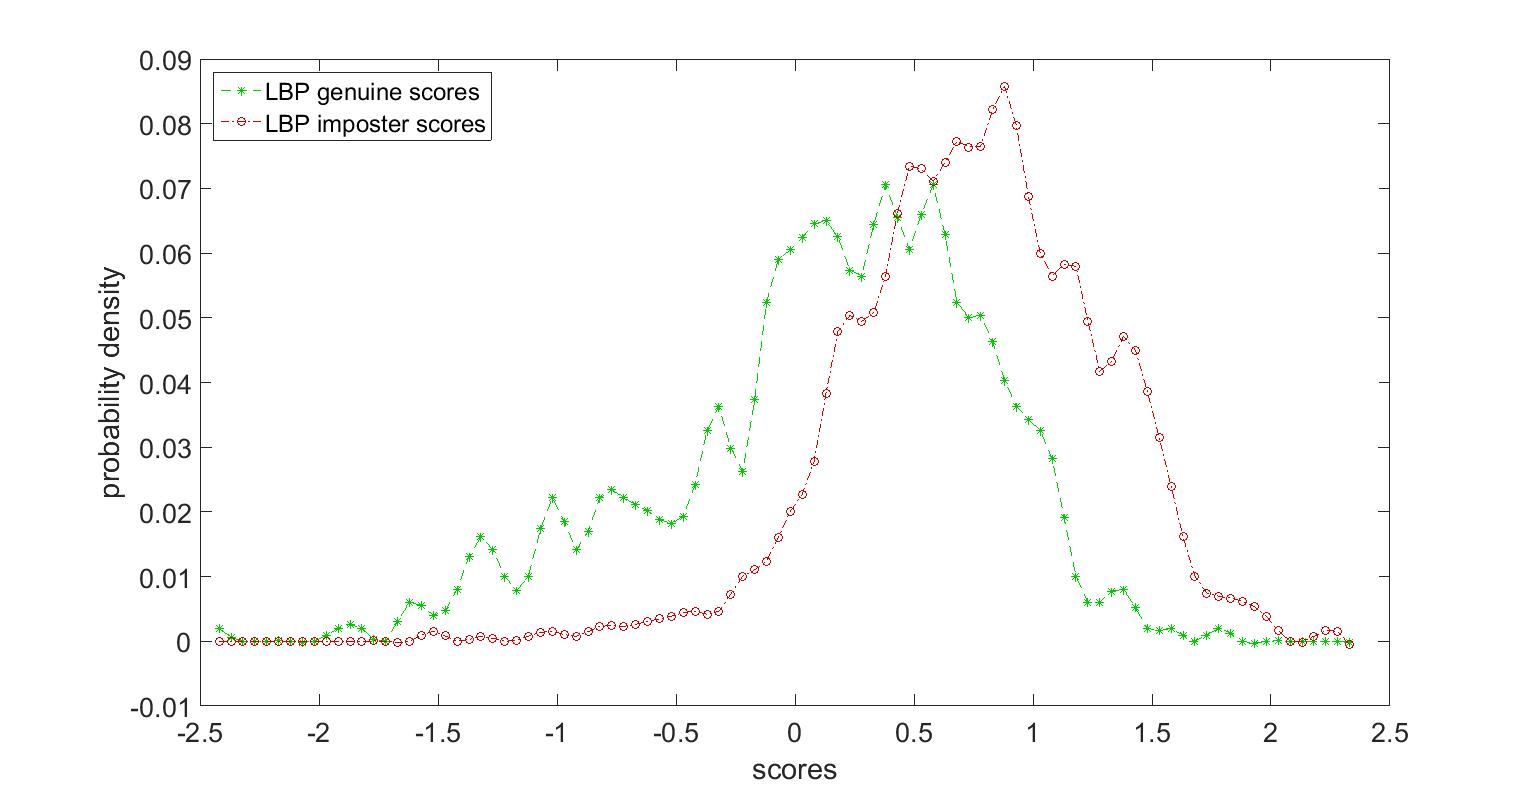
\includegraphics[width=\textwidth]{LBP.jpg}
        \caption{LBP = $78.04\%$}
        \label{fig:LBP}
    \end{subfigure}
    \begin{subfigure}[b]{0.44\textwidth}
        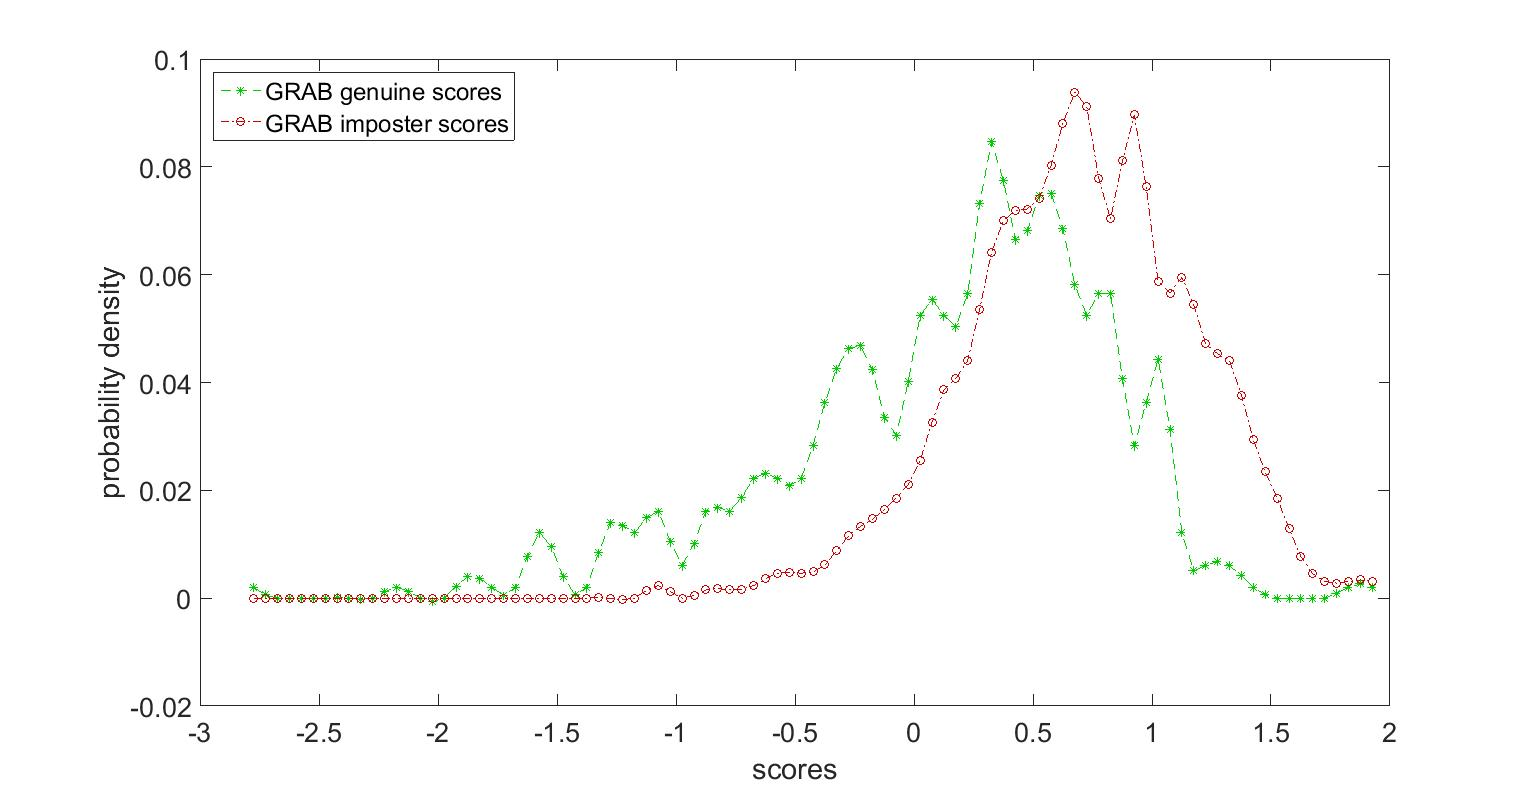
\includegraphics[width=\textwidth]{GRAB.jpg}
        \caption{GRAB = $76.59\%$}
        \label{fig:GRAB}
    \end{subfigure}
        \begin{subfigure}[b]{0.44\textwidth}
        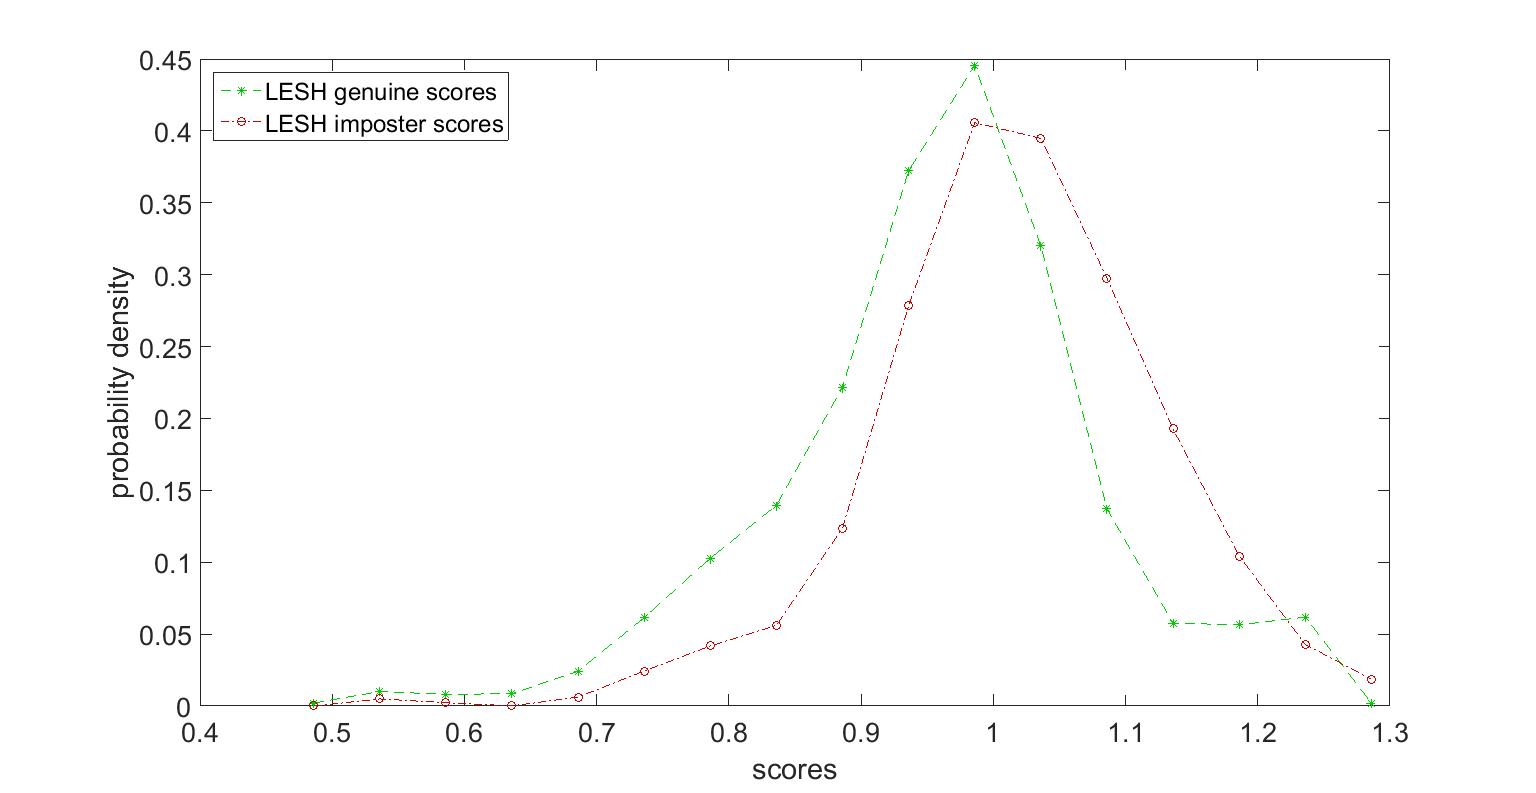
\includegraphics[width=\textwidth]{LESH.jpg}
        \caption{LESH = $72.29\%$}
        \label{fig:LESH}
    \end{subfigure}
    \begin{subfigure}[b]{0.44\textwidth}
        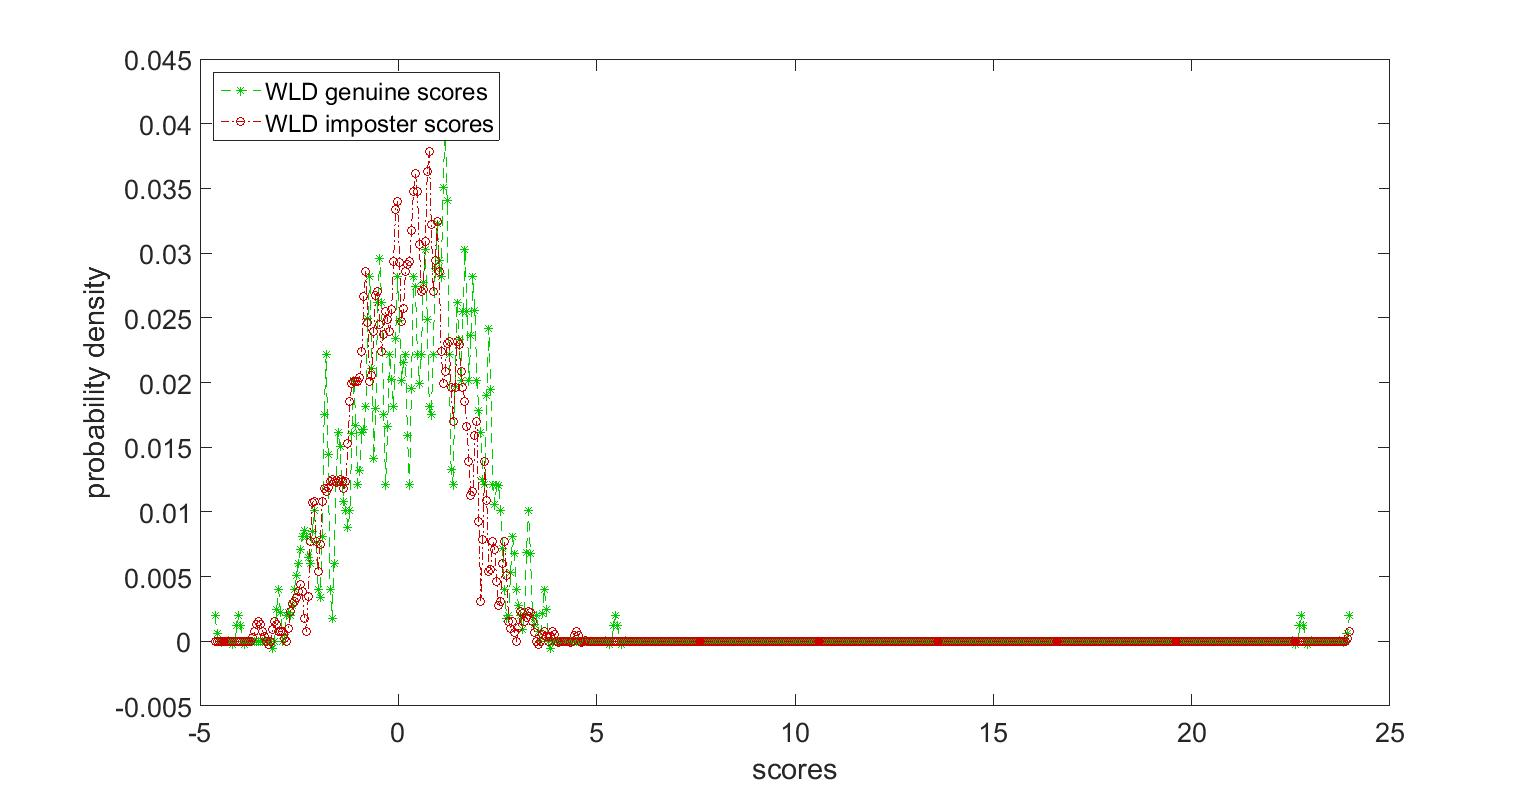
\includegraphics[width=\textwidth]{WLD1.jpg}
        \caption{WLD = $60.22\%$}
        \label{fig:WLD}
    \end{subfigure}
    \centering
    \caption{ Probability Density distribution wrt similarity scores of feature extractors in descending order of the classification accuracy}\label{fig:pds}
\end{figure}

\begin{figure}[H]
    \centering
    \begin{subfigure}[b]{0.2\textwidth}
        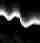
\includegraphics[width=\textwidth]{CC01.jpg}
        \caption{}
    \end{subfigure}
    \begin{subfigure}[b]{0.2\textwidth}
        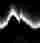
\includegraphics[width=\textwidth]{CC02.jpg}
        \caption{}
    \end{subfigure}
    \begin{subfigure}[b]{0.2\textwidth}
        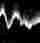
\includegraphics[width=\textwidth]{CC03.jpg}
        \caption{}
    \end{subfigure}
    \begin{subfigure}[b]{0.2\textwidth}
        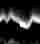
\includegraphics[width=\textwidth]{CC04.jpg}
        \caption{}
    \end{subfigure}
    \caption{Correctly classified Mine data}\label{fig:cc0}
\end{figure}

\begin{figure}[H]
    \centering
    \begin{subfigure}[b]{0.2\textwidth}
        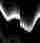
\includegraphics[width=\textwidth]{WC01.jpg}
        \caption{}
    \end{subfigure}
    \begin{subfigure}[b]{0.2\textwidth}
        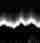
\includegraphics[width=\textwidth]{WC02.jpg}
        \caption{}
    \end{subfigure}
    \begin{subfigure}[b]{0.2\textwidth}
        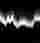
\includegraphics[width=\textwidth]{WC03.jpg}
        \caption{}
    \end{subfigure}
    \begin{subfigure}[b]{0.2\textwidth}
        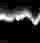
\includegraphics[width=\textwidth]{WC04.jpg}
        \caption{}
    \end{subfigure}
    \caption{Misclassified Mine data}\label{fig:wc0}
\end{figure}

\begin{figure}[H]
    \centering
    \begin{subfigure}[b]{0.2\textwidth}
        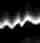
\includegraphics[width=\textwidth]{CC11.jpg}
        \caption{}
    \end{subfigure}
    \begin{subfigure}[b]{0.2\textwidth}
        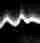
\includegraphics[width=\textwidth]{CC12.jpg}
        \caption{}
    \end{subfigure}
    \begin{subfigure}[b]{0.2\textwidth}
        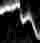
\includegraphics[width=\textwidth]{CC13.jpg}
        \caption{}
    \end{subfigure}
    \begin{subfigure}[b]{0.2\textwidth}
        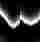
\includegraphics[width=\textwidth]{CC14.jpg}
        \caption{}
    \end{subfigure}
    \caption{Correctly classified Rock data}\label{fig:cc1}
\end{figure}

\begin{figure}[H]
    \centering
    \begin{subfigure}[b]{0.2\textwidth}
        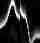
\includegraphics[width=\textwidth]{WC11.jpg}
        \caption{}
    \end{subfigure}
    \begin{subfigure}[b]{0.2\textwidth}
        
\includegraphics[width=\textwidth]{WC12.jpg}
        \caption{}
    \end{subfigure}
    \begin{subfigure}[b]{0.2\textwidth}
        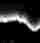
\includegraphics[width=\textwidth]{WC13.jpg}
        \caption{}
    \end{subfigure}
    \begin{subfigure}[b]{0.2\textwidth}
        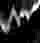
\includegraphics[width=\textwidth]{WC14.jpg}
        \caption{}
    \end{subfigure}
    \caption{Misclassified Rock data}\label{fig:wc1}
\end{figure}

%third part of resut section
\subsection{Discussion}
\tab This section explores probability density curves and patterns distinguishing one class from another. In the first part, scores from Linear-SVM are derived and probability density of these scores are studied. On the other hand, in the second part, images of two classes of rock and mine are scrutinized using our best classification results. 
\\
\tab SVM-Linear classifier outputs scores containing class posterior probability. Only one of the class probability scores are taken into consideration. Positive values of the scores represent a specific category of class while negative values represent the other classes. This aids in segregating the input test data into a genuine or an imposter score. In this case we consider genuine scores to be the predicted rock class and imposter scores as mine class. Plotting the probability density of genuine and imposter scores result in Figure~\ref{fig:pds}. Lesser the overlap between the genuine and imposter curves, better is the performance. From the plots it is evident that, system with higher classification accuracy has lesser over-lapping area than otherwise. Therefore, region of overlap directly relates to the separability of the class. Figure~\ref{fig:pds} (a), (b), (c), and (d) with lesser region of overlap excel at separating the data into a rock or a mine. 

\tab Careful analysis of Figure \ref{fig:cc0},\ref{fig:wc0},\ref{fig:cc1} and \ref{fig:wc1} indicate pattern inherent to the rock and the mine classes. Mis-Classified results are derived from HOG+LPQ fused features and Linear-SVM classifier. From the figures, rock data signals are found to be flatter than mine data signals, with exceptions of Figure \ref{fig:wc0} (a), \ref{fig:cc1} (c) and \ref{fig:wc1} (c). Using larger datasets, should improve the classification results by reducing anomalies. Further, HOG and LPQ might have managed to capture this probable distinguishing pattern between a rock and a mine.

%conclusion and future work
\section{Conclusions}
\tab In this paper, we propose HOG to be the most efficient feature extractor in classifying landmine signals. HOG calculates gradient orientations in a dense overlapping grid. Landmine signals vary with respect to spatial orientations, which is strongly captured by HOG features. LPQ which uses phase information, is also blur invariant. Thus the fusion of LPQ and HOG features adequately capture the distinctive pattern of a rock and a mine. This result can be generalized only with rigorous data collection and experimentation under dynamic conditions. 
\\
\\
\begin{large}
\textbf{Future Work:}
\end{large}
Getting access to the larger dataset should improve performance with GRNN and SVM-RBF classifiers. Also, study of feature extractors involving extended dataset, could help infer detailed data patterns. Additionally, research can be further extended to use key-point feature descriptor to reduce input feature dimensions. Lastly, modifying existing feature extractors by tweaking their internal mathematical flow could help us come up with a generic algorithm for the landmine data.

\bibliographystyle{plain}
\bibliography{bbfile}

\end{document}
